\chapter{Experiments}
\label{chap:experiments}
We implement the multi-bit spike train model with SpikingJelly \cite{doi:10.1126/sciadv.adi1480} using its PyTorch backend, and compare it with the traditional 1-bit spike train model on various tasks and datasets. We investigate the convergence, accuracy, firing rate, and quantizability of the multi-bit spike train model. 

We mainly use the Fashion MNIST dataset \cite{xiao2017/online} and a convolutional neural network (CNN) to set up the experiments of an image classification task. We will also show the results also hold on more complex datasets like CIFAR-10 \cite{Krizhevsky2009}. 

In the following sections, the input images from Fashion MNIST are first converted to spike trains using the Poisson encoding method. The CNN has a structure of $28\times 28 - 8c5 - 2a - 16c5 - 2a - 10o$, visually illustrated in Figure \ref{fig:scnn_structure}. 

\begin{figure}[!htpb]
    \centering
    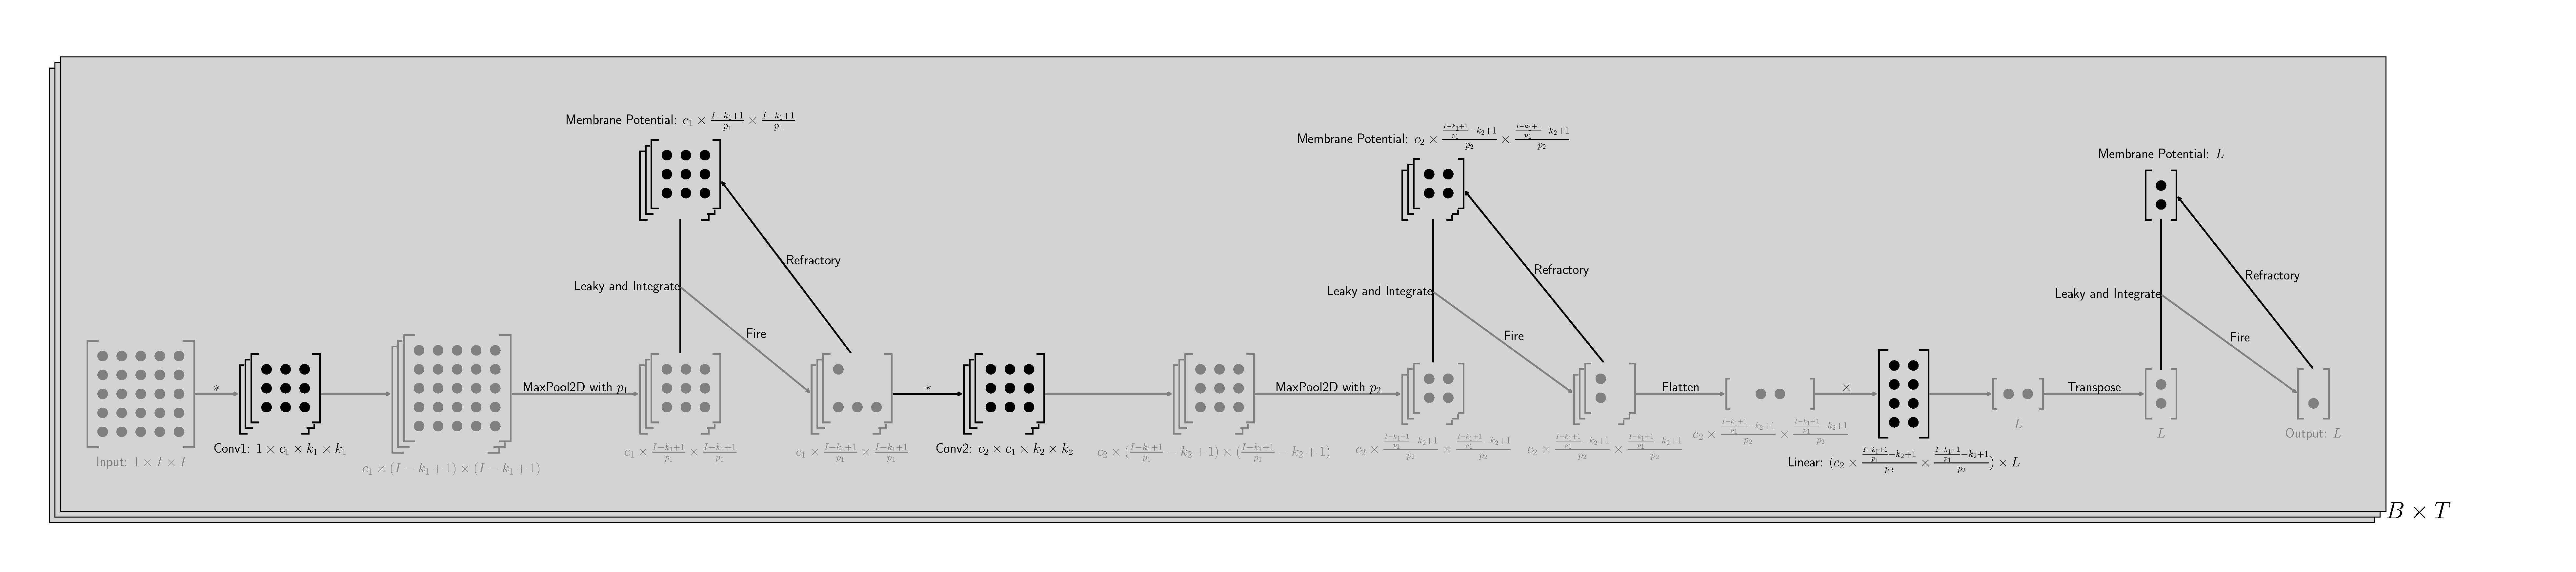
\includegraphics[width=\textwidth]{assets/standard/FashionMNIST/snn.pdf}
    \caption{The CNN structure used in the experiments with Fashion MNIST dataset}
    \label{fig:scnn_structure}
\end{figure}

    \section{Convergence \& Accuracy}
    \label{sec:convergence_accuracy}
        The first noticeable difference between the multi-bit spike train model and the 1-bit spike train model is the convergence speed (see Figure \ref{fig:convergence_speed}). Even just by increasing the bit width of the spike train from 1 to 2, the convergence speed of the network is significantly improved. 
        \begin{figure}[!htpb]
            \centering
            \begin{subfigure}[H]{\textwidth}
                \centering
                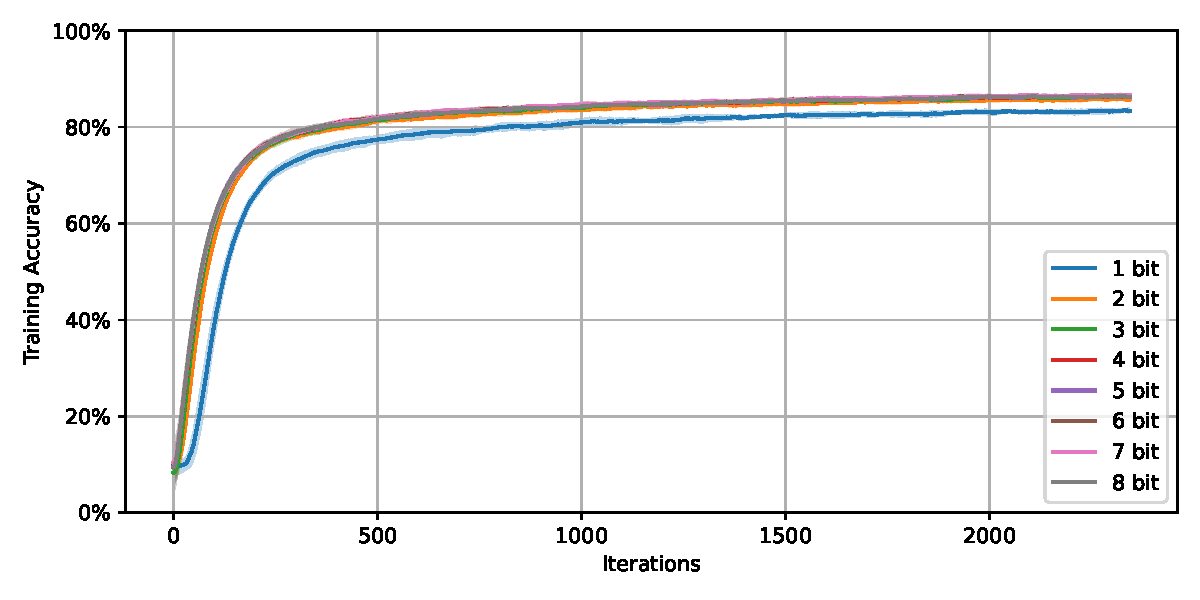
\includegraphics[width=\textwidth]{../standard/FashionMNIST/plots/fashionmnist_train_acc.pdf}
                \caption{Training Accuracy (smoothed with a window size of 100)}
            \end{subfigure}
            \hfill
            \begin{subfigure}[H]{\textwidth}
                \centering
                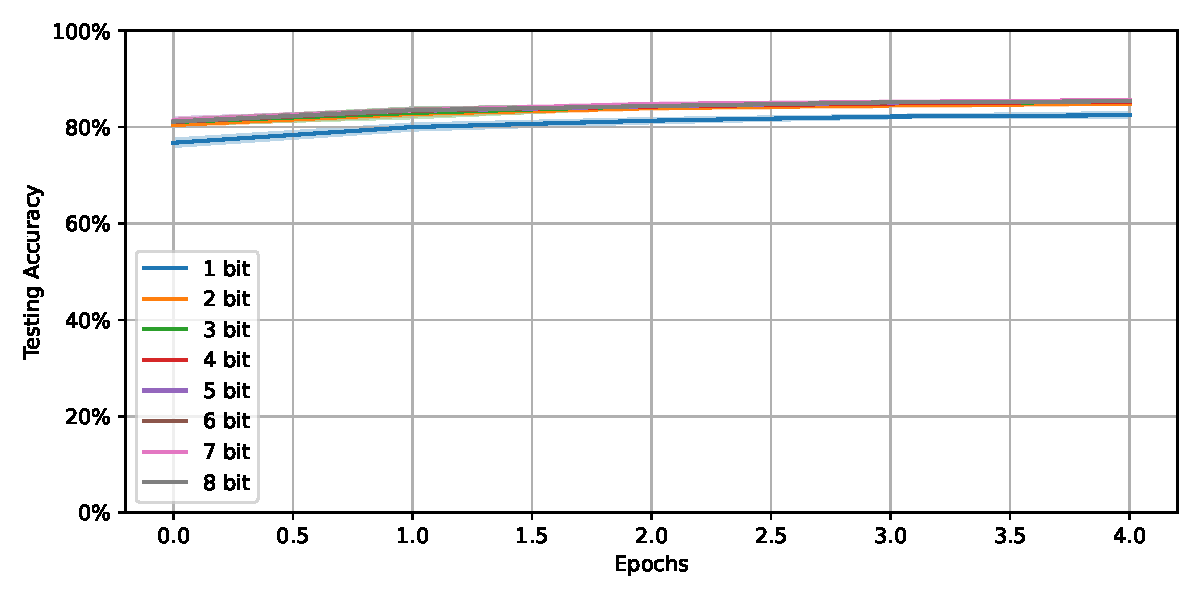
\includegraphics[width=\textwidth]{../standard/FashionMNIST/plots/fashionmnist_test_acc.pdf}
                \caption{Test Accuracy}
            \end{subfigure}
            \caption{Comparison of the Convergence Speed of 1-bit to 8-bit Spike Train Model, repetition of the experiment 10 times}
            \label{fig:convergence_speed}
        \end{figure}

        It may not seem to be much graphically, but the improvement in convergence speed can lead to significant reduction in the training time if considering a fixed target accuracy, especially considering the diminishing return of the training time with respect to the target accuracy. 

        Here we set the target accuracy to be 80\%. The training time of the multi-bit spike train model is reduced by around 50\%, shown in Figure \ref{fig:iterations_fixed_accuracy}. 
        \begin{figure}[!htpb]
            \centering
            \begin{subfigure}[H]{0.47\textwidth}
                \centering
                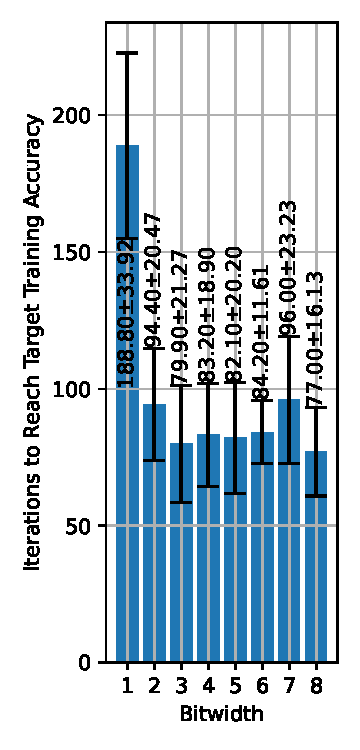
\includegraphics[width=\textwidth]{../standard/FashionMNIST/plots/fashionmnist_train_iters.pdf}
                \caption{Iterations to reach 80\% training accuracy}
            \end{subfigure}
            \hfill
            \begin{subfigure}[H]{0.47\textwidth}
                \centering
                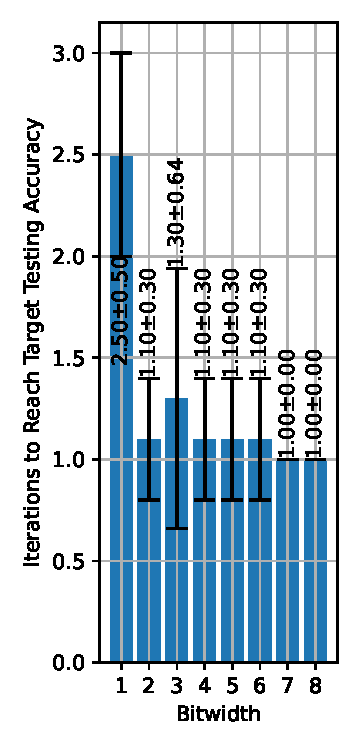
\includegraphics[width=\textwidth]{../standard/FashionMNIST/plots/fashionmnist_test_iters.pdf}
                \caption{Epochs to reach 80\% testing accuracy}
            \end{subfigure}
            \caption{Comparison of the Training Time of 1-bit to 8-bit Spike Train Model, repetition of the experiment 10 times}
            \label{fig:iterations_fixed_accuracy}
        \end{figure}

        Such great improvement however also comes at certain cost:
        \begin{itemize}
            \item The improvement in convergence speed diminishes as the bit width of the spike train increases. The improvement from 2-bit to 3-bit or even higher bit width is not as significant as the improvement from 1-bit to 2-bit.
            \item The more complicated the model is, the harder is it to train the multi-bit spike train model. One can easily run into the problem of overfitting, for example in the case of DVS gesture recognition task.
        \end{itemize}

        Due to the faster convergence speed, the multi-bit spike train model can achieve better accuracy than the 1-bit spike train model given a fixed number of iterations or epochs for the most cases (see Figure \ref{fig:final_accuracy}).
        \begin{figure}[!htpb]
            \centering
            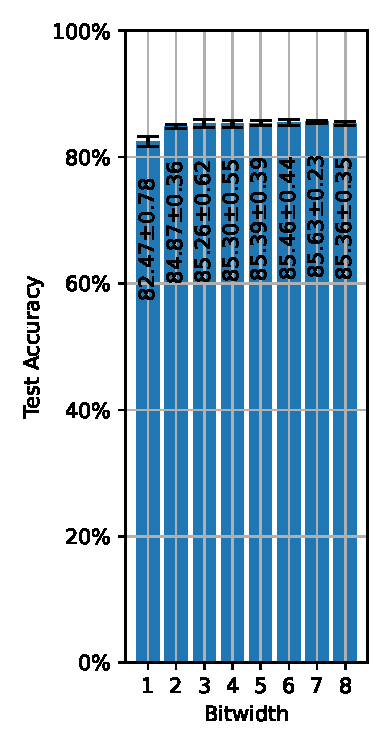
\includegraphics[width=\textwidth]{../standard/FashionMNIST/plots/fashionmnist_final_acc.pdf}
            \caption{Comparison of the Final Accuracy of 1-bit to 8-bit Spike Train Model after 5 epochs, repetition of the experiment 10 times}
            \label{fig:final_accuracy}
        \end{figure}

        In general, such behaviors can be shown on MNIST \cite{deng2012mnist}, NMNIST \cite{10.3389/fnins.2015.00437}, Fashion MNIST, DVS gesture recognition \cite{8100264}, and CIFAR-10 datasets (see Appendix \ref{appendix:accuracy}).

    \section{Firing Rate}
    \label{sec:firing-rate}
        SNNs are known for their sparsity in the firing rate of the neurons. Here we notice that the multi-bit spike train model has a higher firing rate than the 1-bit spike train model (see Figure \ref{fig:firing_rate}), as tradeoff for the improvement in convergence speed. 
        \begin{figure}[!htpb]
            \centering
            \begin{subfigure}[H]{0.48\textwidth}
                \centering
                \includegraphics[width=\textwidth]{../standard/FashionMNIST/plots/fashionmnist_train_firerate.pdf}
                \caption{Training Firing Rate}
            \end{subfigure}
            \hfill
            \begin{subfigure}[H]{0.48\textwidth}
                \centering
                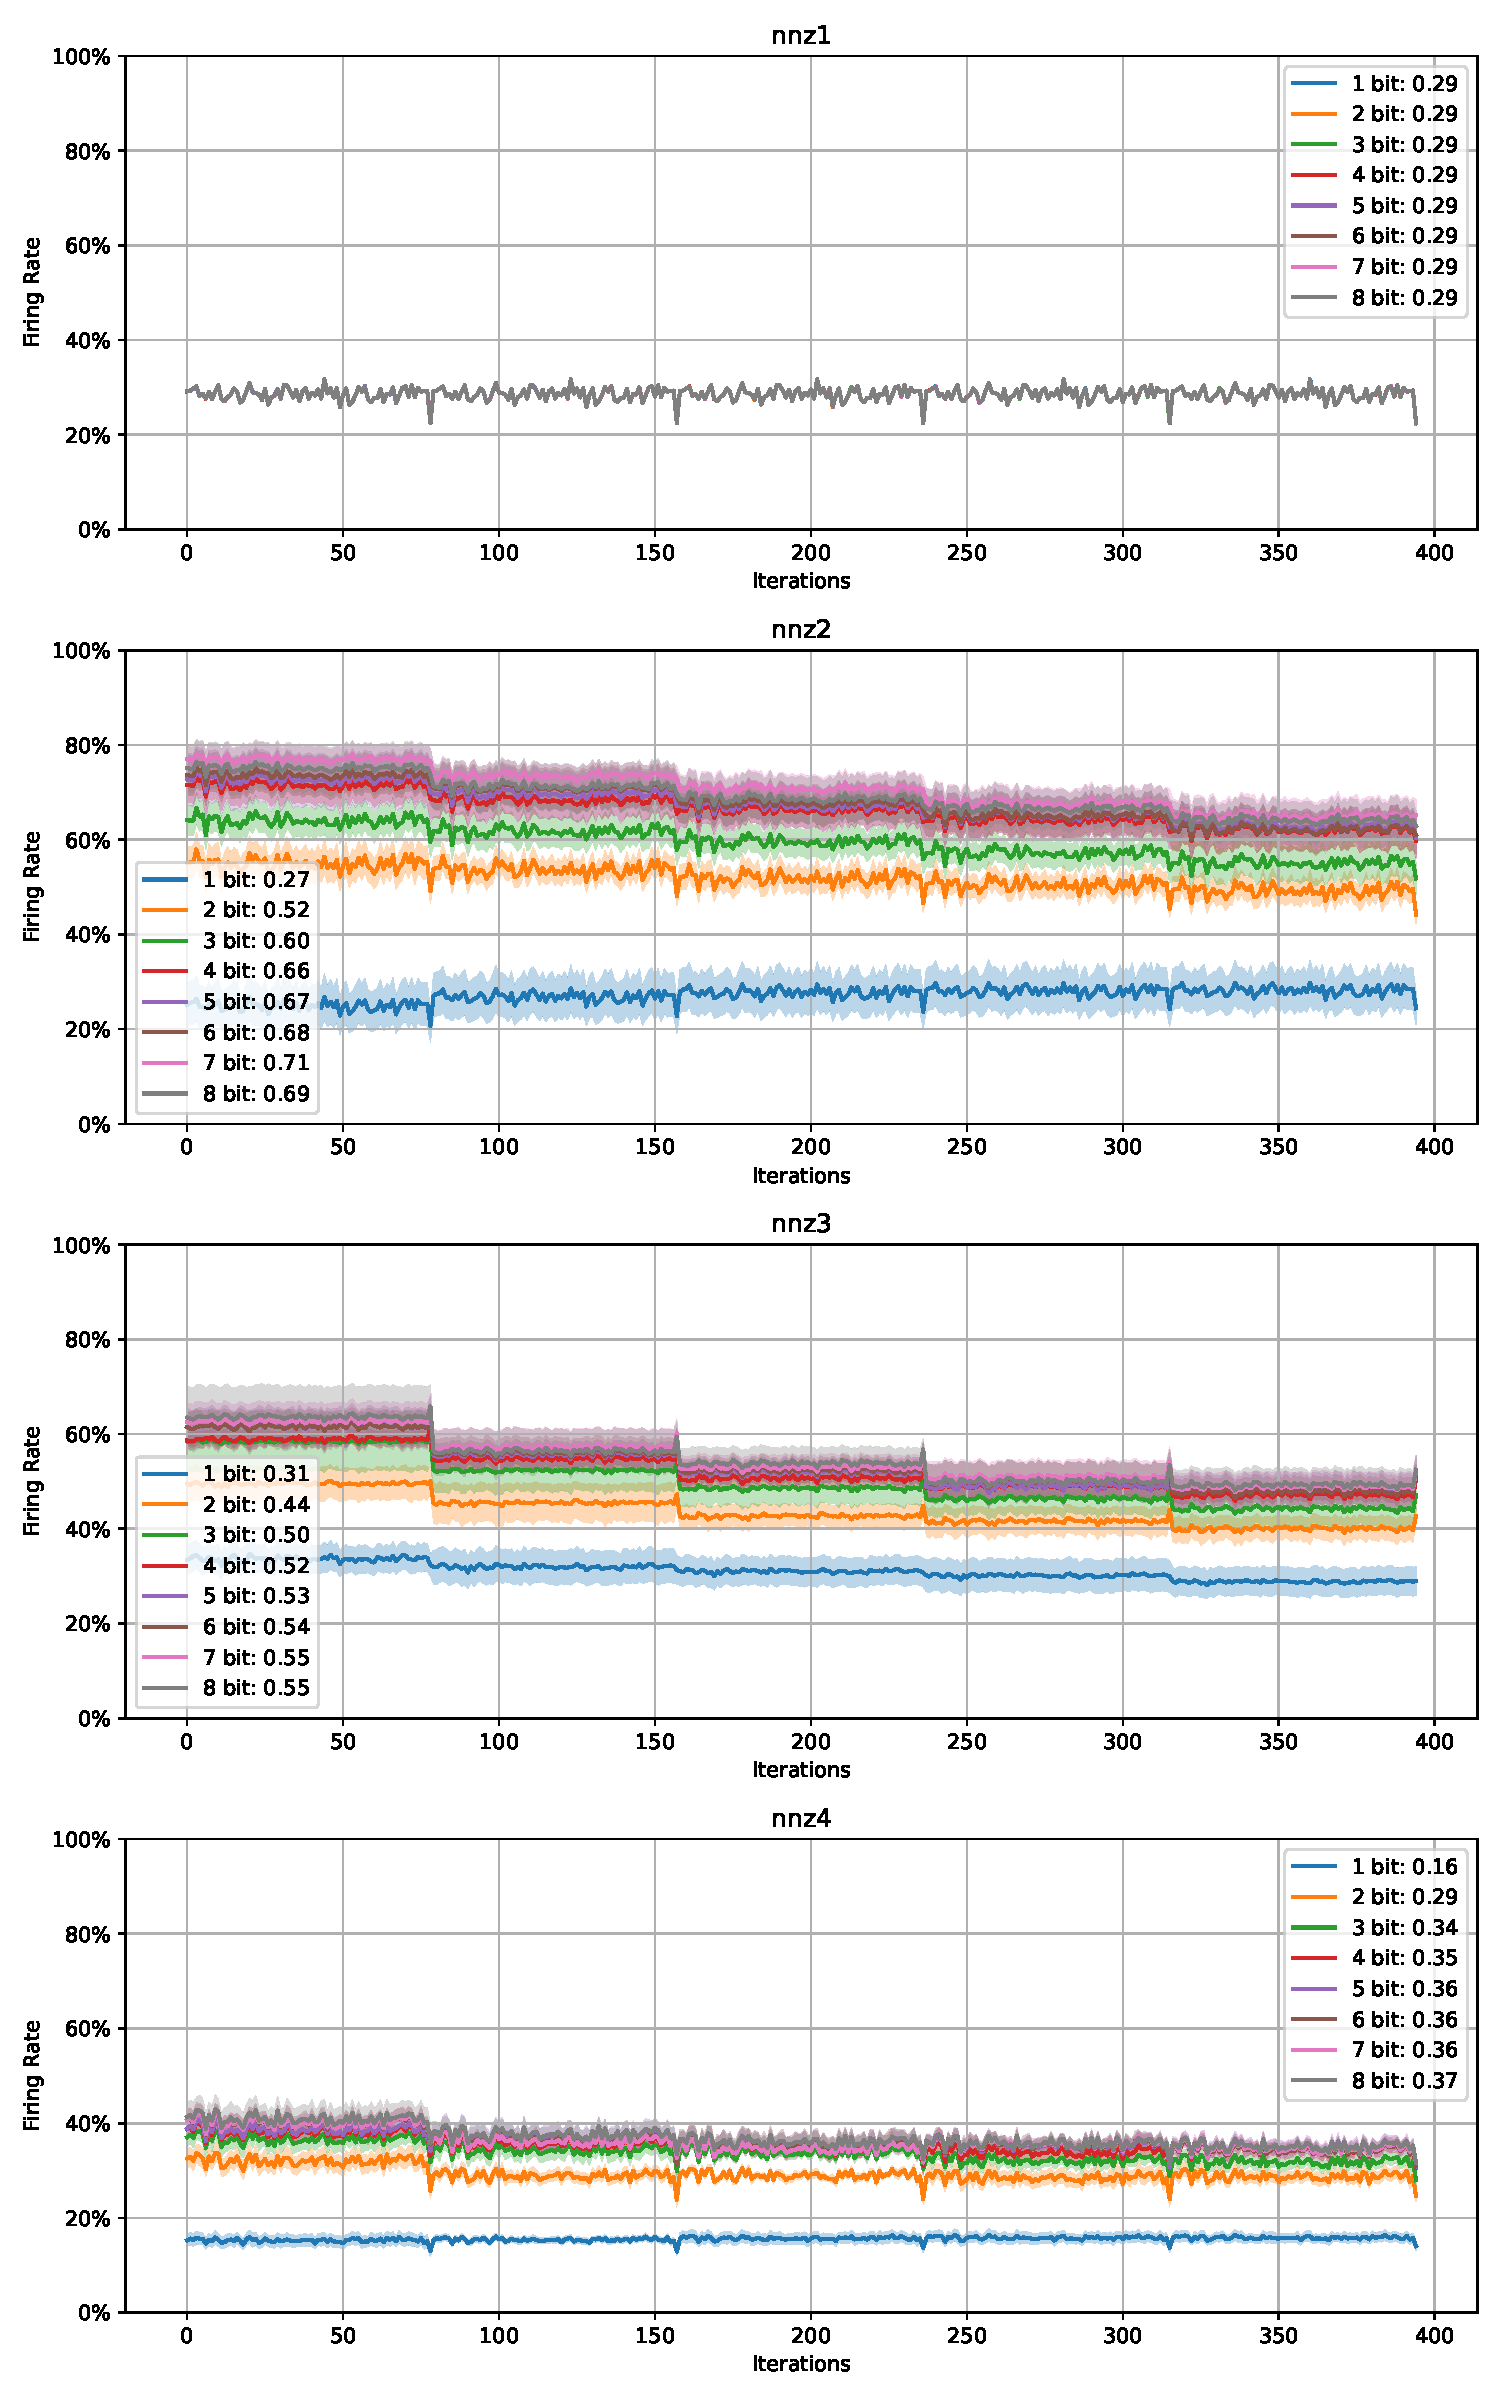
\includegraphics[width=\textwidth]{../standard/FashionMNIST/plots/fashionmnist_test_firerate.pdf}
                \caption{Test Firing Rate}
            \end{subfigure}
            \caption{Comparison of the Firing Rate of 1-bit to 8-bit Spike Train Model: repetition of the experiment 10 times, "nnz[i]" means the number of non-zero elements in the $i$-th measuring point, corresponding to the position from the inputs to the output layer, "nnz1" is the input data}
            \label{fig:firing_rate}
        \end{figure}

        One can notice that the firing rate of the multi-bit spike train model peaks at the very beginning of the training session, when the model converges rapidly. The firing rate then decreases as the training progresses. If we extend the training session, the firing rate of the multi-bit spike train model tends to converge to the firing rate of the 1-bit spike train model. Such process takes however a long time (see Figure \ref{fig:long_firing_rate}). 
        \begin{figure}[!htpb]
            \centering
            \begin{subfigure}[H]{0.48\textwidth}
                \centering
                \includegraphics[width=\textwidth]{../firerate/FashionMNIST/plots/fashionmnist_train_firerate.pdf}
                \caption{Training Firing Rate}
            \end{subfigure}
            \hfill
            \begin{subfigure}[H]{0.48\textwidth}
                \centering
                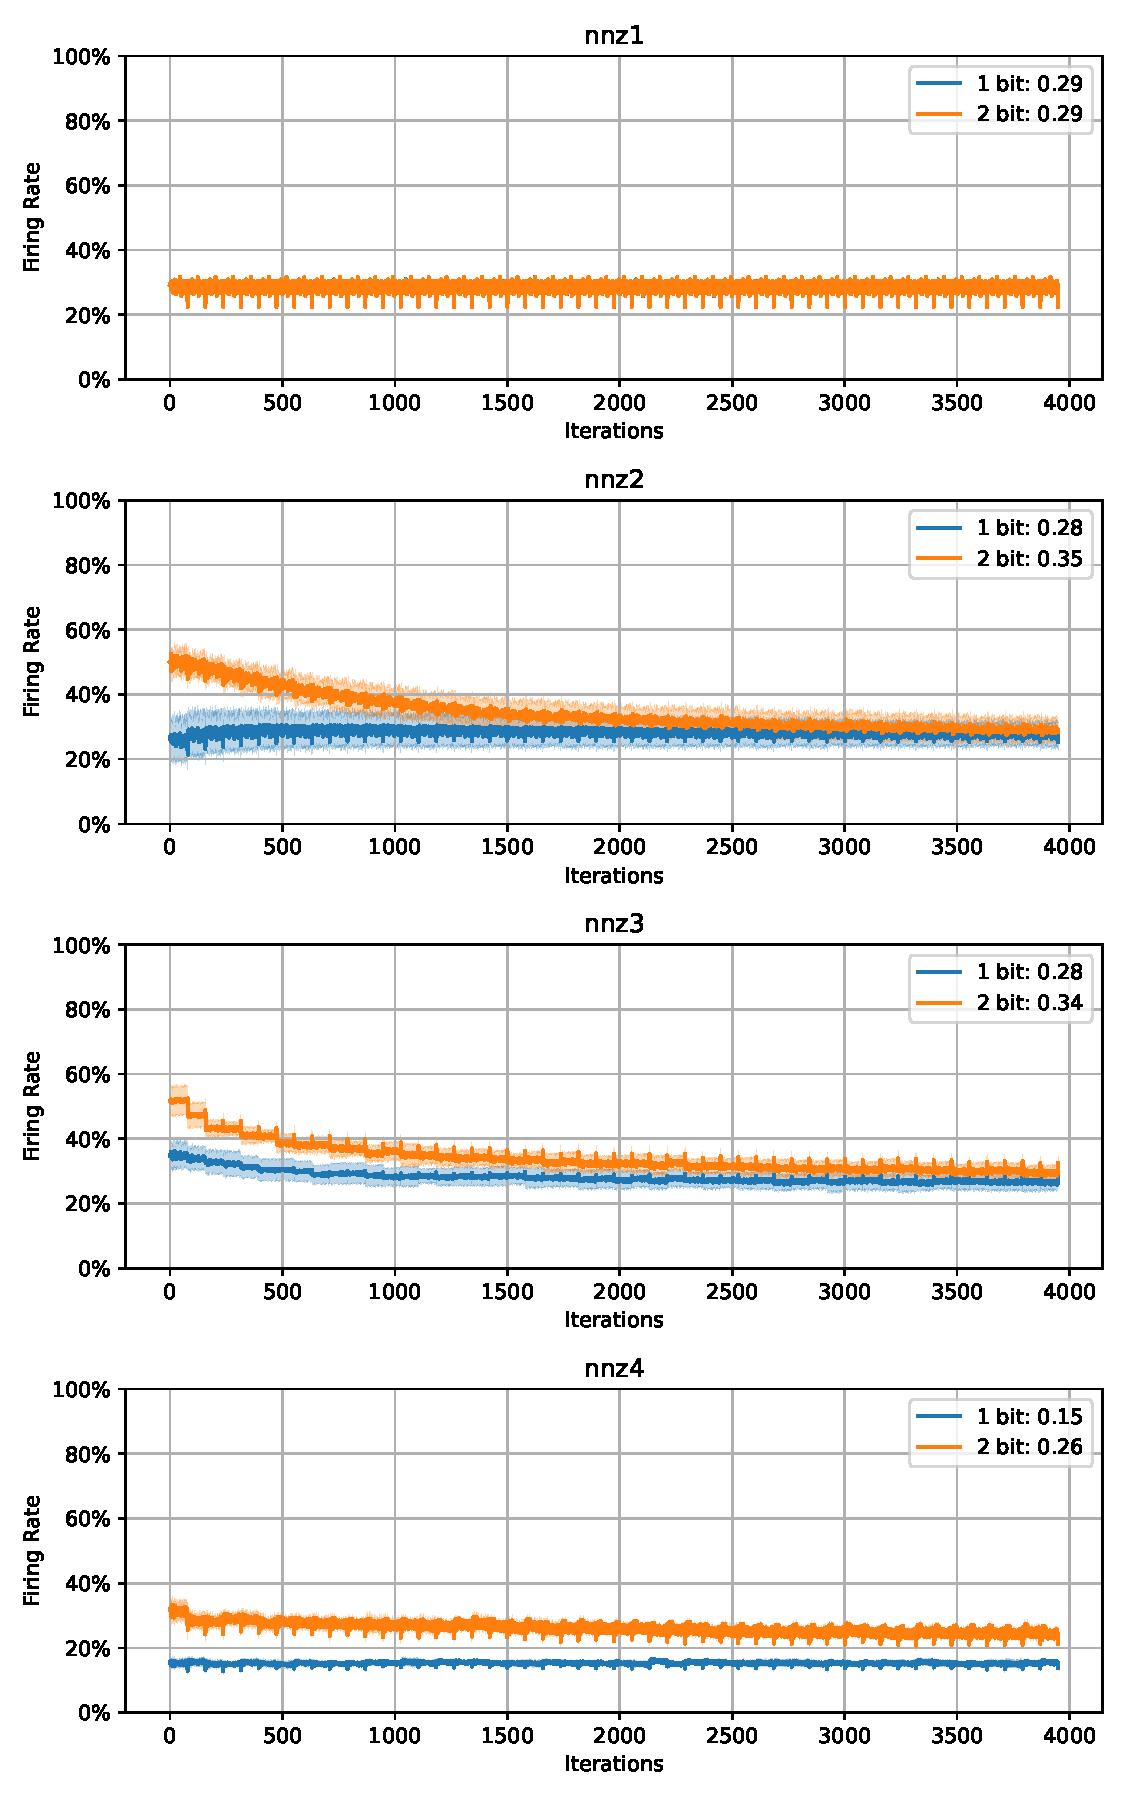
\includegraphics[width=\textwidth]{../firerate/FashionMNIST/plots/fashionmnist_test_firerate.pdf}
                \caption{Test Firing Rate}
            \end{subfigure}
            \caption{Analog to figure \ref{fig:firing_rate}, but with a training session of 50 epochs instead of 5 epochs, only the 1-bit and 2-bit spike train models}
            \label{fig:long_firing_rate}
        \end{figure}

        In the end, the firing rate of the multi-bit spike train model is comparable to the 1-bit spike train model (see Figure \ref{fig:final_firing_rate}).
        \begin{figure}[!htpb]
            \centering
            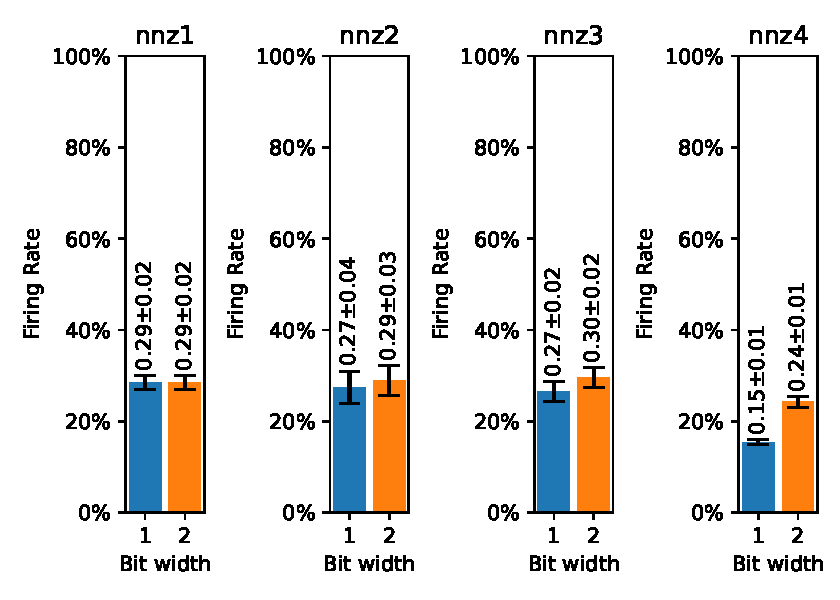
\includegraphics[width=\textwidth]{../firerate/FashionMNIST/plots/fashionmnist_final_firerate.pdf}
            \caption{Comparison of the Final Firing Rate of 1-bit to 8-bit Spike Train Model after 50 epochs, only the 1-bit and 2-bit spike train models}
            \label{fig:final_firing_rate}
        \end{figure}

        Such behavior is more visible on simpler datasets like MNIST. For now, we do not have any explanation for this phenomenon (see Appendix \ref{appendix:firerate}).

    \section{Quantizability}
    \label{sec:quantizability}
        It is well known that SNNs are easy to quantize. There are studies showing that the weights and activations of SNNs can be quantized to 1-bit or 2-bit without significant loss in accuracy. Here we show that both the multi-bit spike train model and the 1-bit spike train model can be trained with \verb|bf16| and quantized to \verb|int8| without significant loss in accuracy.
        % TODO: Add references to the studies showing the quantizability of SNNs
        \begin{figure}[!htpb]
            \centering
            \begin{subfigure}[H]{0.48\textwidth}
                \centering
                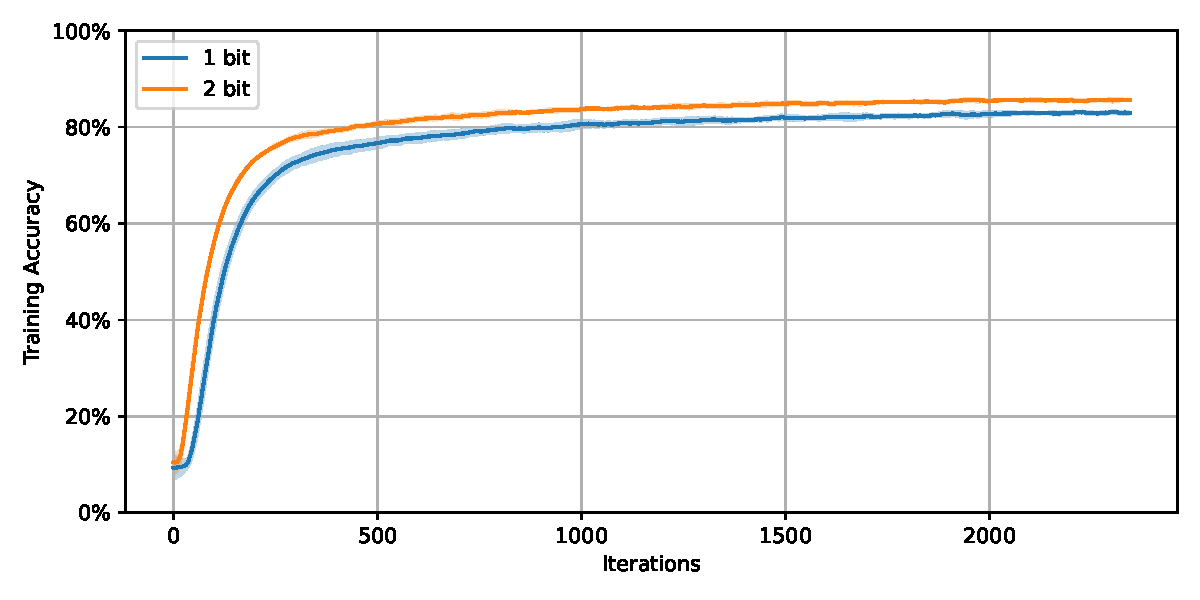
\includegraphics[width=\textwidth]{../quantized/FashionMNIST/plots/fashionmnist_train_acc.pdf}
                \caption{Training Accuracy with half precision (smoothed with a window size of 100)}
            \end{subfigure}
            \hfill
            \begin{subfigure}[H]{0.48\textwidth}
                \centering
                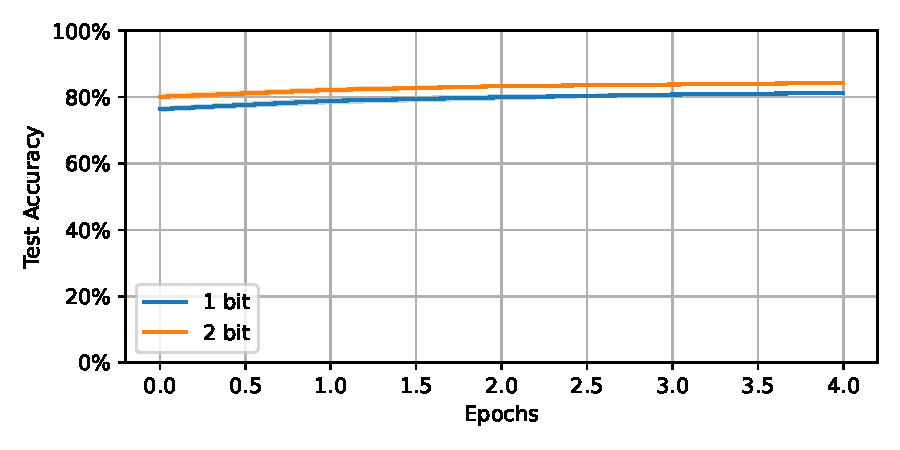
\includegraphics[width=\textwidth]{../bf16/FashionMNIST/plots/fashionmnist_test_acc.pdf}
                \caption{Test Accuracy with half precision}
            \end{subfigure}
            \hfill
            \begin{subfigure}[H]{\textwidth}
                \centering
                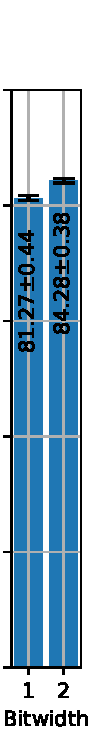
\includegraphics[width=\textwidth]{../bf16/FashionMNIST/plots/fashionmnist_final_acc.pdf}
                \caption{Final Accuracy with half precision after 5 epochs}
            \end{subfigure}
            \caption{Comparison of the Convergence Speed of 1-bit to 8-bit Spike Train Model with half precision, repetition of the experiment 10 times}
            \label{fig:half_precision}
        \end{figure}

        As shown in Figure \ref{fig:half_precision}, both SNN models converge well as if they were trained with \verb|float32|. Meanwhile the multi-bit spike train model has its advantage in the convergence speed and accuracy preserved. 
       
        Before quantizing the models to \verb|int8|, we first apply quantization-aware training to both SNN models. While regular ANNs may encounter various problems, both SNN models here converge well. We also see that the multi-bit spike train model has a faster convergence speed and better accuracy than the 1-bit spike train model (Figure \ref{fig:quantization_aware}). 
        \begin{figure}[!htpb]
            \centering
            \begin{subfigure}[H]{0.48\textwidth}
                \centering
                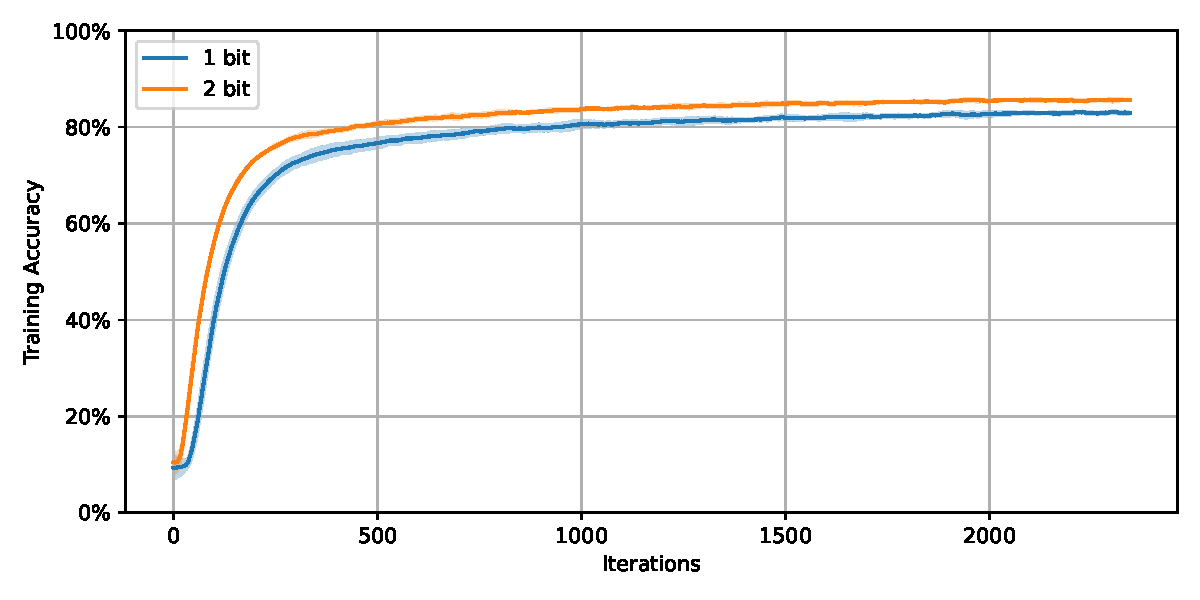
\includegraphics[width=\textwidth]{../quantized/FashionMNIST/plots/fashionmnist_train_acc.pdf}
                \caption{Training Accuracy with quantization-aware training (smoothed with a window size of 100)}
            \end{subfigure}
            \hfill
            \begin{subfigure}[H]{0.48\textwidth}
                \centering
                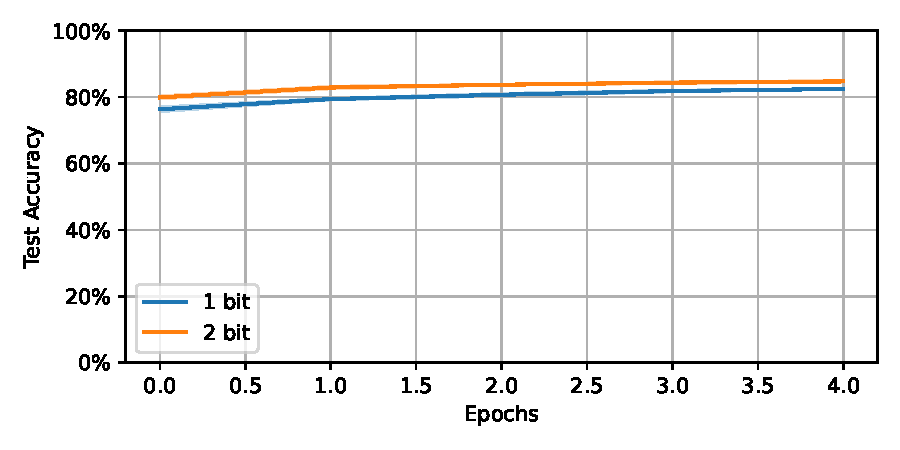
\includegraphics[width=\textwidth]{../quantized/FashionMNIST/plots/fashionmnist_test_acc.pdf}
                \caption{Test Accuracy with quantization-aware training}
            \end{subfigure}
            \hfill
            \begin{subfigure}[H]{\textwidth}
                \centering
                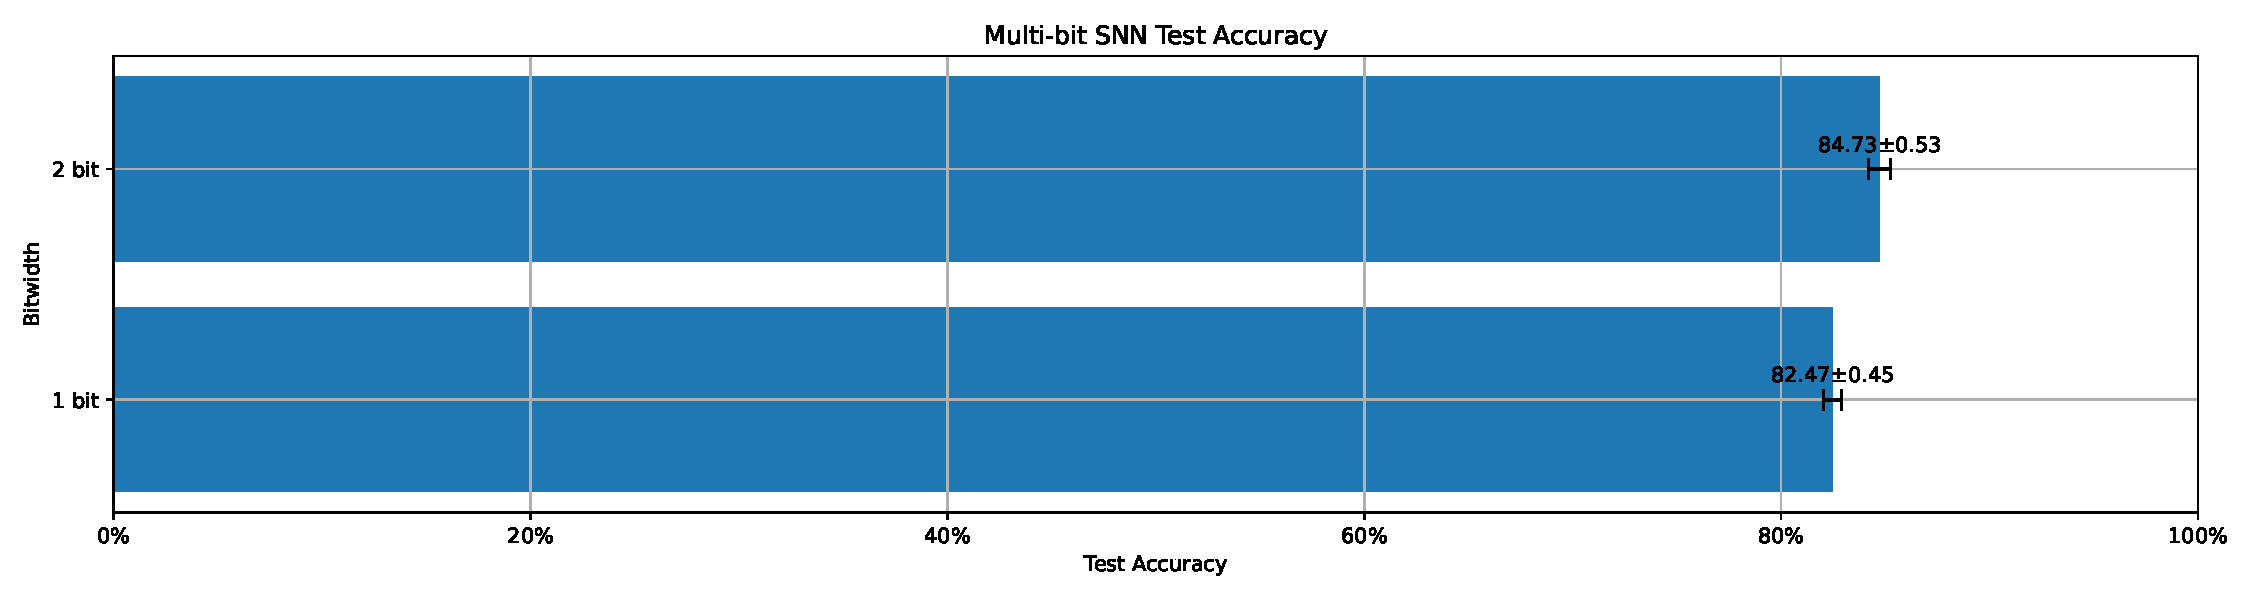
\includegraphics[width=\textwidth]{../quantized/FashionMNIST/plots/fashionmnist_final_acc.pdf}
                \caption{Final Accuracy with quantization-aware training after 5 epochs}
                \label{fig:quantization_aware_final_acc}
            \end{subfigure}
            \caption{Comparison of the Convergence Speed of 1-bit to 8-bit Spike Train Model with quantization-aware training, repetition of the experiment 10 times}
            \label{fig:quantization_aware}
        \end{figure}

        We then quantize the weights and biases to \verb|int8| using the PyTorch quantization API. The quantization of the LIF layer is not supported at the moment. We evaluate the quantized models on the test set. The final accuracy is barely affected by the quantization (see Figure \ref{fig:quantization_aware_final_acc}). 